\section{LSST Strategy for Discovering Solar System Objects} 

We briefly describe the LSST system design and observing strategy, and discuss in more
detail image processing and moving object detection. 

\subsection{A Brief Overview of LSST  Design} 

LSST will be a large, wide-field ground-based optical telescope system
designed to obtain multiple images covering the sky that is visible
from Cerro Pach\'{o}n in Northern Chile. The current baseline design,
with an 8.4m (6.7m effective) primary mirror, a 9.6 deg$^2$ field of
view, and a 3.2 Gigapixel camera, will allow about 10,000 square
degrees of sky to be covered every night, with typical 5$\sigma$ depth 
for point sources of $r\sim24.5$ (AB). The system is designed to yield 
high image quality (the median delivered seeing in the $r$ band of 
about 0.8 arcsec) as well as superb astrometric  and photometric 
accuracy\footnote{For detailed specifications, please see the LSST
Science Requirements Document, http://ls.st/srd}. The total survey
area will include $\sim$30,000 deg$^2$ with $\delta<+34.5^\circ$, and 
will be imaged multiple times in six bands, $ugrizy$, covering the 
wavelength range 320--1050 nm. The project is scheduled to  begin the 
regular survey operations at the start of next decade. 

LSST will be operated in fully automated survey mode. About 90\% of the 
observing time will be devoted to a deep-wide-fast survey mode which will 
uniformly observe a 18,000 deg$^2$ region about 1000 times (summed over 
all six bands) during the anticipated 10 years of operations, and yield a coadded map 
to $r\sim27.5$. These data will result in catalogs including about
$40$ billion stars and galaxies, that will serve the majority of the
primary science programs. The remaining 10\% of the observing time
will be allocated to special projects such as a Very Deep and Fast
time domain survey\footnote{Informally known as ``Deep Drilling Fields".}.



\subsection{LSST Observing Strategy} 

As designed and funded (by the U.S National Science Foundation and
Department of Energy), LSST is primarily a science-driven mission. 
The LSST is designed to achieve goals set by four main science themes:
\begin{enumerate}
\item Probing Dark Energy and Dark Matter;
\item Taking an Inventory of the Solar System;
\item Exploring the Transient Optical Sky;
\item Mapping the Milky Way.
\end{enumerate}
Each of these four themes itself encompasses a variety of analyses, with 
varying sensitivity to instrumental and system parameters. These themes 
fully exercise the technical capabilities of the system, such as photometric 
and astrometric accuracy and image quality. 

The current baseline survey strategy is planned to maximize the overall science returns, including 
Solar System science, rather than NEO/PHA discovery completeness (though the 
two goals are highly interrelated). Discovering and linking objects in the Solar System 
moving with a wide range of apparent velocities (from several degrees per day for 
NEOs to a few arc seconds per day for the most distant TNOs) places strong 
constraints on the cadence of observations. The baseline strategy requires closely 
spaced pairs of observations, two or preferably three times per lunation. The visit
exposure time is set to 30 seconds to minimize the effects of trailing for the majority of 
moving objects. The images are well sampled to enable accurate astrometry, with 
anticipated absolute accuracy of at least 0.1 arcsec.

LSST observations can be simulated using the LSST Operations Simulator tool (OpSim, XXX give
reference here). OpSim runs a survey simulation with given science-driven desirables, 
a software model of the telescope and its control system, and models of weather and other 
environmental variables. The output of such a simulation is an ``observation history'', which 
is a record of times, pointings and a record of associated environmental data and telescope  
activities throughout the simulated survey.  This history can be examined to assess  
the efficacy of the simulated survey for any particular science goal or 
interest\footnote{For examples of such analysis, see http://ls.st/xpr}. 


\subsection{LSST Baseline Survey Strategy}

As the system understanding improves, the baseline survey strategy and the telescope model 
gets updated, generally on a yearly schedule. The current reference baseline survey is known 
as {\it minion\_1016}. It includes 2.4
million visits collected over 10 years, with 85\% of the observing time spent on the 
main survey and the rest on various specialized programs. The median number of visits
{\it per night} is 816, with 3,026 observing nights. The median airmass is 1.23 (the
minimum altitude for LSST telescope if 20 deg.). In the $r$ band, the median seeing 
(FWHM) is 0.81 arcsec, and the median $5\sigma$ depth for point sources is 24.16 
(using the best current estimate of the fiducial depth at airmass of one of 24.39). 

There are a few known problems with this simulation, including twilight sky brightness
estimates that are too bright, the moon avoidance is not as aggressive as it could be,
and observations are biased towards west, away from the meridian. The implied impact
of these shortcomings on NEO completeness estimates is a few percent (the performance 
of this simulated cadence in NEO context is discussed in detail in \S5). An improved simulation, 
that will presumably rectify these problems, will become available by the end of 2017. 


\subsection{Overview of LSST  Data Management and Image Processing} 

The images acquired by the LSST Camera will be processed by LSST Data Management
software \citep{juric15} to a) detect and characterize imaged
astrophysical sources and b) detect and characterize temporal changes
in the LSST-observed universe. The results of that processing will be
reduced images, catalogs of detected objects and their measured properties, and 
prompt alerts to ``events'' -- changes in astrophysical scenery discovered by differencing 
incoming images against older, deeper, images of the sky in the same direction ({\em
templates}). More details about the main algorithms and pipeline design are available
in Appendix~\ref{sec:AppA}. 

LSST will use two methods to detect moving objects in difference images: 
\begin{enumerate}
\item Detecting trailed motion on the sky: objects trailed by more
  than 2 PSF widths (corresponding to motion faster than about 1
  deg/day) will be easily detectable as trailed.  Two trailed
  detections within 20--60 minutes in a single night will be
  sufficient to identify an object as an NEO candidate,
\item Inter-night linking of pairs: this technique will recover
  objects moving too slow enough to be measurably elongated in 
  a single exposure. 
\end{enumerate} 

We note that sources detected in difference images (DIASources in LSST parlance, see Appendix~\ref{sec:AppA})
will also include false detections, colloquially known as {\it false positives}. 
In addition to false positives due to instrumental artifacts and software glitches, 
in this context they will also include detections of true astrophysical transients 
(e.g. gamma-ray burst afterglow) that will not be associated with static sources
(e.g. stars and galaxies). Estimates of expected false positive rates are discussed
in \S\ref{sec:imDiff}. 



\subsection{The Basic Strategy for Linking Detections into Orbits} 

The LSST strategy for linking detections into orbits assumes the following main steps
\begin{enumerate}
\item Detections in difference images (obtained during the same night), that are not 
    associated with static objects (e.g. variable stars) within a small exclusion radius 
    (a fraction of an arcsec), are linked into tracklets.
\item At least three tracklets obtained in a 15-30 day wide window are linked into 
         candidate tracks.
\item Candidate tracks are filtered (pruned from false tracks) using the initial orbit 
         determination (IOD) 
\end{enumerate}

False positives, be it false detections, false tracklets or false tracks, are assumed not be 
an issue because IOD will efficiently and reliably filter out false tracks due to high-accuracy 
astrometry and well-understood simple Keplerian model predictions. Therefore, the 
essential question is whether the resulting number of false tracks, and the corresponding
IOD step, can be handled with available computing resources.

Assuming 0.005 sec per IOD (based on an analysis by Pan-STARRS MOPS team,
reference XXX; possibly shorter now?), a 1000-core machine, and 12 hours of computation 
time per day, one can filter about 10$^{10}$ candidate tracks per day. How many tracks 
can be plausibly expected? 

MOPS tests and analytic considerations show that with of the order a 
million tracklets per night (similar to the expected rate, with false positives included, 
as demonstrated below), a 30-day search window results in about the same number of 
tracks per night as input tracklets. Assuming 2 million tracklets per night, a 30-day 
search window would result in about 60 million candidate tracks. This expectation is more 
than two orders of magnitude smaller than the assumed system capacity above. Additionally, 
as discussed below in more detail, the number of false tracks could be decreased by another 
order of magnitude by decreasing the mean revisit time to 10 minutes. 



\begin{verbatim}
We want to explain 
1) why does the number of tracklets found by MOPS scale with the square 
of the number of false positives, and 
2) why is the number of tracks similar to the number of tracklets. 
\end{verbatim}



\subsection{Expected False Tracklet Rates \label{sec:tracklets} }

Given a detection in the difference image,  another difference image, obtained at a different epoch, 
is searched for a matching detectio to form a tracklet. For orientation, the sky 
density of asteroids down to LSST $5\sigma$ faint flux limit ($r \sim 24.5$) is of the order 
$\rho_{ast} \sim 100$ deg$^{-2}$. The predicted highest asteroid sky density for $r<24.5$, 
on the Ecliptic, is up to about five times larger (with an uncertainty of about a factor of 2, 
depending on model assumptions), and the density decreases rapidly with the ecliptic latitude. 
A typical LSST observing night includes about 1000 visits, with two visits per night over 
the active sky area. The nominal LSST field-of-view area is $A_{FOV}=9.6$ deg$^2$, with a 
fill factor of 0.9, giving an effective field-of-view area of $A_{FOV}^{eff}=8.64$ deg$^2$. Hence, 
the number of detected asteroids per night is of the order 500,000 (with implied two detections 
per asteroid), although it can be significantly lower when the Ecliptic is not well covered (and 
it could be a few times higher if the majority of visits were obtained along the Ecliptic). 

The number of detections due to (gaussian) background fluctuations, the so-called ``false 
positives'', is about $\rho_{bkgd} = 60$ deg$^{-2}$, assuming typical LSST seeing (0.8 arcsec) 
and SNR$>$5. For a given seeing and SNR threshold, the rate of false positives can never be 
lower than this estimate. This false positive rate decreases with the square of the seeing, and 
strongly depends on SNR: the rate decreases/increases by a factor of about ten when SNR 
threshold is increased/decreased by one (see \S\ref{sec:imDiff}). 

Analysis of DECam images reduced using prototype LSST software, described in \S\ref{sec:imDiff},  
shows a higher rate of detections in difference images, and a fraction of those detections 
cannot be readily associated with true moving objects. This analysis implies a conservative 
upper limit for the false positive rate of about $\rho_{FP} =  400$ deg$^{-2}$. This value 
is an upper limit because analyzed DECam fields are close to the Ecliptic, with a significant but
not well known contribution from real asteroids (due to very faint flux levels, $r \sim 24$),
and it also includes true astrophysical transients that are not associated with static objects
(stars and galaxies). It is quite possible that the false positive rate might be as much as four 
times lower, though we will proceed with the most conservative estimate above. 

We will assume that the sky density of detections in difference images, $\rho_{det}$, is given by 
the sum of contributions from true asteroids and false positives, $\rho_{det} = \rho_{ast} + \rho_{FP}
= 500$ deg$^{-2}$. When searching for a matching detection in another difference image, there are
two distinct types of behavior. Correct matches of detections of the same asteroids into tracklets follow the behavior 
expected for correlated samples: as long as the object's angular displacement between the two epochs 
is sufficiently larger than the seeing disk, while at the same time smaller than the search radius, the
number of matches (that is, the number of true tracklets produced per LSST pointing, assuming 
two visits of the same area per night) is simply 
\begin{equation}
                  N_{tracklet}^{true} = \rho_{ast}  \, A_{FOV}^{eff},
\end{equation}
With  $\rho_{ast} = 100$ deg$^{-2}$, $N_{tracklet}^{true} \sim 1,000$ per a pair of visits, and with
500 visit pairs per typical observing night, $N_{tracklet}^{true} \sim 500,000$ per night (same as 
the number of detected asteroids in the active sky area, of course). Again,
this number can be much lower for fields far away from the Ecliptic, and a few times larger
for exceptionally good coverage of the Ecliptic. We emphasize that this number of true tracklets 
does not directly depend on the search radius, nor the time elapsed between the two visits, as long 
as they have their plausible values (about an arcminute, and a few tens of minutes, as discussed 
further below). 

There are three other types of tracklets that follow behavior for uncorrelated (random) 
samples: associations of different asteroids, associations of asteroids and false detections, 
and tracklets made of two false detections. Assuming the same $\rho_{det}$ in both 
difference images, for each of $N_{det} = \rho_{det} \, A_{FOV}^{eff}$ detections in one image,
we search for a matching detection in another image. The search radius is given by 
$\delta_{max} = v_{max} \, \Delta t$. Here $v_{max}$ is the  cutoff velocity and $\Delta t$ 
is the time elapsed between the two images. For LSST baseline cadence, $\Delta t$ is in 
the range 20-60 minutes. The search area, $A_S = \pi \delta_{max}^2$, is then 
\begin{equation}
     A_S = 0.0055 \left( v_{max}  \over {\rm deg \, day}^{-1} \right)^2 \, \left(\Delta t \over {\rm hour} \right)^2 {\rm deg}^2.
\end{equation}
Adopting $v_{max} = 1$ deg day$^{-1}$, which ensures a high completeness level even for fast-moving 
NEOs\footnote{Simulations imply that 95\% of NEO detections have $v<1$ deg day$^{-1}$; with this threshold,
the completeness for main-belt asteroids is essentially 100\%. Objects moving faster than 1 deg day$^{-1}$ will
be easily resolved in LSST images and can be treated separately using specialized algorithms.}, and $\Delta t = 30$
minutes (which together  imply a search radius of $\delta_{max} = 1.3$ arcmin), gives a search area of 
$A_S = 0.0014$ deg$^2$. 

As long as $\rho_{det}$ is smaller than $\rho_A = 1/A_S = 733$ deg$^{-2}$, the expected number of 
matches within the search radius is less than unity (for a discussion of second-order effects, see Appendix B 
in \citealt{IVLZ2005}). In this regime, the probability of forming a tracklet is well described by 
\begin{equation}
                 p_{tracklet}^{false} =   { \rho_{det}  \over \rho_A}, 
\end{equation}
and the total expected number of {\it false} tracklets is 
\begin{equation}
           N_{tracklet}^{false} = N_{det} \, p_{tracklet}^{false} =  \rho^2_{FP}  \, A_S \, A_{FOV}^{eff} \,
                                \left(1 + 2 \eta + \eta^2\right),
\end{equation}
where $\eta = \rho_{ast}  / \rho_{FP} \sim 0.25$. With $\rho_{ast} = 100$ deg$^{-2}$ and  $\rho_{FP} = 400$ deg$^{-2}$, 
$N_{tracklet}^{false} \sim 3,000$ per pair of visits, and $N_{tracklet}^{false} \sim 1.5$ million per observing night with 
500 visit pairs. We note that the density of false tracklets (350 deg$^{-2}$) is similar to $\rho_{FP}$; this similarity
is a consequence of choosing $\delta_{max}$ such that $\rho_{FP} A_S \sim 1$. 

The first term is the largest and corresponds to tracklets made of two false detections ($\sim1.0$ million), 
the second term corresponds to associations of asteroids and false detections, and the third and the smallest term 
($<0.1$ million) is due to incorrect associations of different asteroids.

The total number of tracklets is thus up to about 2 million per observing night, for the chosen parameter 
values. Given that these choices are rather conservative, this estimate is essentially an upper limit; approximately, 
{\it we expect of the order a million tracklets per observing night}. We note that these false positive estimates imply that
the detection SNR threshold could be decreased from 5 to 4 without detrimental effects on the false positive rate:
while this SNR change would increase the number of false positives due to background fluctuations by about a factor of 10
(from about 60 deg$^{-2}$ to about 600 deg$^{-2}$), the total number of false positives would not increase by more
than about a  factor of 2.  Analysis discussed in \S\ref{sec:opsim} shows that such a change of SNR threshold would increase 
the NEO completeness by  about 2\%. 

To the first order ($\eta \approx 0$)
\begin{equation}
   N_{tracklet} =  N_{tracklet}^{true} + N_{tracklet}^{false} = \rho_{ast}  \, A_{FOV}^{eff} + \rho^2_{FP}  \, A_S \, A_{FOV}^{eff}. 
\end{equation}
In addition to $N_{tracklet}^{false}$ scaling with the square of $\rho_{FP}$, $N_{tracklet}^{false}$ scales with the square of
both $v_{max}$ and  $\Delta t$ (via the dependence on $A_S$). Therefore, if $\Delta t$ would be made
as small as 10 minutes by modifying observing strategy, the resulting $N_{tracklet}^{false}$ would be about an 
order of magnitude smaller (and $N_{tracklet}$ about three times smaller).  Hence, the shortening of $\Delta t$ is 
a good mitigation strategy against high false positive detection rates in difference images\footnote{An
extreme example of this mitigation strategy would be to obtain two consecutive 30-second visits with
their mid-exposure times separated 
by 34 seconds (additional 2 seconds due to shutter motion and another 2 seconds due to readout). 
The acceptable false positive density would be increased by about three orders of magnitude, with the
lower limit for the detectable motion of the order 0.1 deg day$^{-1}$.}. 



\subsubsection{Can MOPS handle a million tracklets per night?} 

Given $\sim$10$^6$ tracklets per night, how many tracks can be formed in a 30-day search window? 
Based on MOPS test runs described in \S\ref{sec:mops}, we should expect well below 10$^8$ candidate
tracks. LSST's 1000-core system will be capable of easily handling about 10$^{10}$ IODs per day, so we 
have a margin of about two orders of magnitude. Hence, {\it even if the false positive rate in difference 
images is ten times higher than expected, it can still be handled without a change of baseline cadence.} 
Quantitatively, the false positive rates of up to about 4000 deg$^{-2}$ could be readily handled with 
anticipated LSST compute power. For comparison, \cite{denneau13} reported a false positive 
rate of 8,200 deg$^{-2}$ for Pan-STARRS1 project. 

In addition, another factor of a few increase in the false positive rate can be mitigated by a simple
shortening of the revisit time by about a factor of 3. At the same time, an order of magnitude 
larger false positive rates for LSST than measured using DECam images and prototype LSST software
are rather implausible. If the LSST camera, or other system component, would somehow
cause such high false positive rates, the whole LSST mission would indeed be a failure. 

Therefore, the LSST strategy for discovering moving Solar System objects will be successful
 if the following three conditions are met
\begin{enumerate}
\item The LSST system hardware and image differencing software performance will result in false positive 
          rates not significantly exceeding $\rho_{FP} =  400$ deg$^{-2}$, estimated here using DECam data
          and LSST prototype software (as detailed in the next section). 
\item Given a 1000-core machine and 12 hours of compute time, MOPS will be able to handle about 
          a million tracklets per night to produce up to about 10$^8$ tracks per 30-day window. 
\item IOD can be executed in 0.005 sec per trial (implying that about 10$^{10}$ candidate tracks can
          be filtered per day). 
\end{enumerate}



\newpage

\subsection{Expected False Track Rates \label{sec:tracks} }


Given the true and false tracklet rates per night,  $N_{tracklet}^{true}=5\times10^5$ and $N_{tracklet}^{false}=
1.5\times10^6$, we seek to estimate the number of false candidate tracks. We assume that the search 
window is $N_w= 30$ days wide, and with $N_{tracklet} = 2\times10^6$ per night, there are $6\times10^7$
tracklets. With about 4,300 deg$^2$ (500 pairs of visits) of sky observed each night, the average density of 
(all) tracklets is $\rho_{tracklet} = 450$ deg$^{-2}$. Assuming that on average the same field is 
revisited every $T_{revisit}=3$ days, the active area includes about 13,000 deg$^2$ of sky. 


\subsubsection{The Tracklet Motion Vector Accuracy} 
 
In addition to its mean position at the mean epoch, each tracklet constrains the motion vector. 
Typical astrometric errors for LSST detections will range from 50 mas at SNR=100 to 150 mas at 
SNR=5. For simplicity, we will assume hereafter that the astrometric errors are $\sigma_a=150$ mas 
for all detections, or $\sim 100$ mas per coordinate. With a temporal separation of two detections in 
a tracklet of $\Delta t$, the motion vector is measured with an accuracy per coordinate of 
\begin{equation}
\label{eq:sigv}
          \sigma_v = 3.6 \, \left({\rm hour} \over \Delta t\right) \,\,\, {\rm arcsec} \, {\rm day}^{-1}.
\end{equation}
With a typical $\Delta t = 30$ min, and assuming a linear motion in each ecliptic coordinate (longitude
$\lambda$ and latitude $\beta$), each coordinate can be predicted at time $t$ with an accuracy of  
\begin{equation}
          \sigma_x = 7.2 \, \Delta k \,\,\, {\rm arcsec} \, {\rm day}^{-1}.
\end{equation}
where $\Delta k$, in days, is the elapsed time between the mean tracklet epoch and time $t$. 
For example, when $\Delta k = 7$ days, $\sigma_x = 50$ arcsec, which is roughly the same 
as the typical detection separation in a tracklet, and comparable to typical distance between
two tracklets. 


\subsubsection{Naive Linking of Tracklets into Candidate Tracks} 

Given a $N_w= 30$ days wide search window, and the middle tracklet, out of three tracklets
needed for a candidate track, positioned on day $k$, $k=2\dots29$, there are $(k-1)(30-k)$
different ways to combine three observing nights. Summing over all possible values of $k$
gives 4060 combinations (for $N_w= 15$ days, there are 455 combinations) 

The expectation value for the number of matches in a search radius corresponding to $3\sigma_x$ 
is given by
\begin{equation}
       N_{match}(\Delta k) = \pi \, (3 \sigma_x)^2 \, \rho_{tracklet} = 
                     0.051 \, (\Delta k)^2 \, \left( \rho_{tracklet}  \over 450 \, {\rm deg}^{-2} \right).
\end{equation}
It follows that the total number of candidate tracks, per single trial tracklet, is
\begin{equation}
\label{eq:Ntt}
       N_{tracklet}^{tracks} = \left( \rho_{tracklet}  \over 450 \, {\rm deg}^{-2} \right)^2 \, \left({0.051 \over T_{revisit}}\right)^2 \, 
               \sum_{k=2}^{N_w-1} \sum_{j=1}^{k-1} \sum_{l=k+1}^{N_w} \, (k-j)^2 \, (l-k)^2. 
\end{equation}
The two terms in the sum reflect the multiplication of the number of matches found on a preceeding
night with the number of matches found on a subsequent night. With $N_w= 30$ days and 
$T_{revisit}=3$ days, $N_{tracklet}^{tracks} \sim 5,000$!  

This naive matching results in a prohibitively large number of candidate tracks: with 
$N_{tracklet} = 2\times10^6$, the number of candidate tracks per search window is 
$N_{w}^{tracks} = 10^{10}$. Even with $N_w= 15$ days, $N_{tracklet}^{tracks} \sim 39$
and $N_{w}^{tracks} \sim 10^{8}$, which is at least a magnitude larger than obtained in 
MOPS experiments. 



\subsubsection{Using Tracklet Motion Vector to Prune Candidate Tracks} 

The naive matching described above only used the motion vector for the middle tracklet to 
predict the positions of the two potential matching tracklets in other nights. While the 
measured motion vectors, hereafter velocities, of the other two matching tracklets were not 
used, they contain valuable information. False tracklets have essentially randomly distributed 
velocities with a cutoff given by $v_{max}$ (recall that $v_{max} = 1$ deg day$^{-1}$ was adopted 
above). The differential velocity distribution for false tracks increases linearly with the
velocity modulus. On the contrary, the velocity of true tracklets is highly correlated with both 
the velocities of the other two true tracklets, as well as the velocities implied by the positions 
of tracklets and their temporal separation. If we define $v_{12}$ and $v_{23}$ to be the latter, and 
$v_1$, $v_2$ and $v_3$ to be measured velocities for each tracklet, then all five values
have to be consistent within some tolerance. A situation where $v_3$ is inconsistent with
other four velocities is illustrated in Figure~\ref{fig:TrackSlide1}.  



\begin{figure}[th!]
\centering
\vskip -2.6in
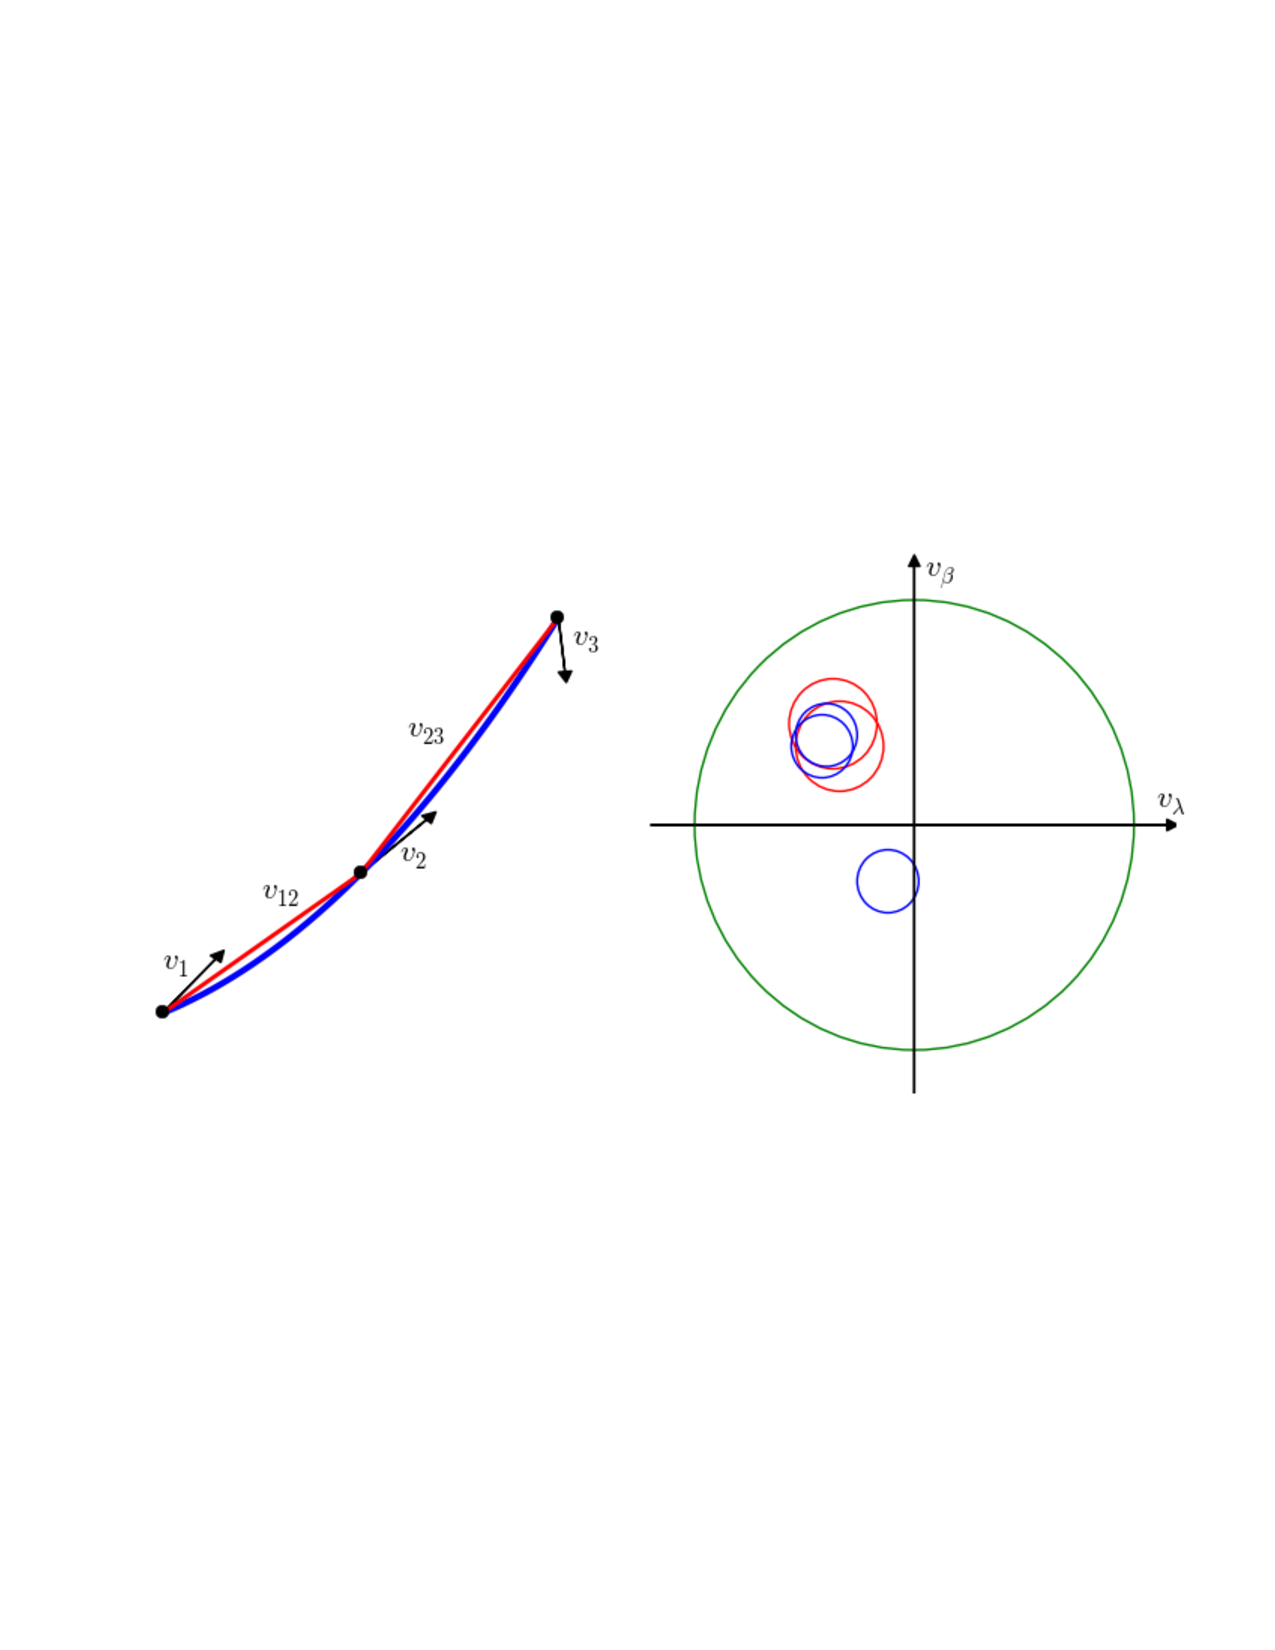
\includegraphics[width=0.95\textwidth]{figures/TrackSlide1}
\vskip -2.7in
\caption{The left panel defines two different types of velocities for a hypothetical asteroid
trajectory shown by the curved blue line. Three tracklets are shown by the black dots; the 
two individual detections per tracklet are not shown, but are implied by the three measured
motion vectors ($v_1$, $v_2$ and $v_3$). The other two velocities ($v_{12}$ and $v_{23}$)
are defined by connecting the pairs of tracklets.  These five velocities are shown in 
ecliptic coordinate system on the right. The circle signifies the cutoff velocity for forming
tracklets. Note that the third tracklet has a velocity that is inconsistent with other four
velocities. The consistency radii are discussed in the text.
\label{fig:TrackSlide1}}
\end{figure}



If the orbital trajectory were a straight line, the velocities would have to align within
their measurement errors. The tracklet velocities ($v_1$, $v_2$ and $v_3$) are measured with 
a precision of about 0.001 deg day$^{-1}$ (see eq.~\ref{eq:sigv}), and $v_{12}$ and $v_{23}$ even 
more precisely due to much larger temporal baselines (a few days instead of fraction of an hour). 
It turns out that the plausible consistency tolerances are driven by orbital curvature and 
acceleration. Analysis of simulated samples\footnote{See Figure 16 in http:/ls.st/LDM-156}
shows that an adequate acceleration limit is 0.02 deg day$^{-2}$: essentially all main-belt
asteroids and more than 95\% of NEOs satisfy this criterion. For a typical 7-day separation
of two tracklets, the implied velocity tolerance is 0.14 deg day$^{-1}$. 


Given that false tracklets have randomly distributed velocities with a cutoff of 1 deg day$^{-1}$,
the probability that a false-tracklet velocity will be consistent with a true velocity is 
(0.14/1.0)$^2 \sim 0.02$. In reality, this probability is a bit smaller because the false-tracklet
velocity distribution is not uniform (it is biased towards the velocity cutoff). Finally, 
the probability that both the first and the third tracklet will have velocities consistent with
the middle tracklet's position and velocity is 0.02$^2$ = 0.0004. The naive matching 
results described above have to be corrected by this factor.  With this additional requirement, 
the expected number of false candidate tracks per single trial tracklet is $N_{tracklet}^{tracks} \sim0.5$ 
with $N_w= 30$ days, and $N_{tracklet}^{tracks} \sim0.02$ with $N_w= 15$ days. 

Although MOPS algorithms operate in a different way, these analytic probabilistic considerations 
explain why the number of candidate tracks produced in MOPS experiments stays approximately
the same (to within a factor of two) even when the number of input tracklets per night is increased
by about an order of magnitude. With $N_{tracklet}^{tracks} \sim0.5$, the number of false candidate 
tracks per search window is about $N_{w}^{tracks} = 250,000$ for $N_w= 30$ days, in good
agreement with the results of MOPS simulations\footnote{See the top left panel 
in Figure 21 in http:/ls.st/LDM-156}. 


Note that for sufficiently large density of false positives,  false tracks will start to dominate: 
with the dependence on $\rho_{tracklet}^2$ from eq.~\ref{eq:Ntt}, and another power of 
$\rho_{tracklet}$ due to multiplication by the number of tracklets per night, $N_{w}^{tracks}$
for false tracks scales as $\rho_{tracklet}^3$. For example, with 20 times higher rate of 
false positives from Pan-STARRS1 than assumed here, the number of false tracks would
be about 10$^4$ higher ($\sim$2 billion instead of 250,000), and prohibitively large. 





\newpage 

\subsection{Systematic effects due to varying modeling assumptions}

XXX This section doesn't belong here, but I wanted Steve and Peter to read it and comment. 
More details will come in Lynne's section on cadence optimization... XXX


The leading systematic effects in completeness estimates are: 
\begin{enumerate}
\item NEO vs. PHA difference (the completeness is about $\sim$5\% higher for PHAs than for NEOs) 
\item Different sample definitions: $H<22$ vs. $D>140$m (as shown by \citep{GMS2016}, completeness
           increases by $\sim$5\% when $H$-based criterion is used) 
\item Orbital parameter distribution for the simulated asteroid population (e.g. the Bottke model
             vs. the Granvik model); varying populations contribute completeness uncertainty of about a few percent) 
\item Variations of the ``discovery window'' (e.g., X visit pairs in N nights: changing N from 15 to 30 with X=3 increases
          completeness by about 4\%; changing X from 3 to 4 with N=15 decreases completeness by 6\%). 
\item Variations of the nominal detection threshold (if the detection threshold is changed from the 
          signal-to-noise ratio of 5 or greater to 4 or greater, the completeness is boosted by 2-3\%; 
          the difference between the optimal detection using trailed profile and point-spread-function 
          detection, which is negligible for LSST baseline exposure time of 30 seconds, would be worth 2\%
          in completeness for doubled exposure time). 
\item Sensitivity to details in sky coverage and cadence (e.g. nightly pairs of visits vs. quads of visits;
          requiring quads instead of pairs of visits decreases completeness by 30\% using baseline cadence; 
          about half of that loss can be recovered using cadence simulations that request four visits per night) 
\item Uncertainties when predicting effective image depth (system throughput, variation of the detection efficiency
          with the signal-to-noise ratio, treatment of trailing losses); for a survey that has a completeness above 60\%, 
          each additional 0.1 magnitude of depth for a given survey cadence increases the completeness by another 1\%.
\item Uncertainties when predicting asteroid's apparent flux (albedo distribution, phase effects, photometric variability 
          due to non-spherical shapes, color distributions); assuming an uncertainty of 0.2 mag in the effective 
          limiting magnitude, the corresponding  systematic uncertainty in completeness is about 2\%.)
\item The slope of the asteroid size distribution (current measurement uncertainty of this parameter 
          corresponds to a systematic uncertainty in completeness of about 2\%.)
\item The impact of known objects: assuming that 43\% objects would be discovered by the start of
          LSST survey, \cite{GMS2016} boosted the final PHA completeness for LSST baseline survey by 11\%. 
\end{enumerate} 

Given these systematic effects, a comparison of different simulation results (both for the same system,
and those of different systems, especially systems operating at different wavelengths) has to be undertaken
with due care. It is unlikely that a meaningful quantitative comparison can be pushed beyond a level
of a few percent (and perhaps as much as 10\%). In practice, the completeness of a given operating survey
is best estimated using the object re-discovery rate. 


